\documentclass[french]{rtxreport}

\usepackage{listings}
\usepackage[utf8]{inputenc}

\author{David Pineau}
\title{Documentation Technique}

\rtxdoctype{Documentation Technique}
\rtxdocref{technical\_documentation}
\rtxdocversion{0.4}
\rtxdocstatus{Release}

\rtxdochistory{
0.1 & 16/04/2011 & David Pineau & Traduction de la version anglaise \\
\hline
0.2 & 18/08/2011 & David Pineau & Traduction de la description
                                  d'implémentation du cache         \\
\hline
0.3 & 19/08/2011 & David Pineau & Correction de typographies        \\
\hline
0.4 & 11/09/2011 & Louis Opter & Traduction de «~Compilation des Interfaces~» \\
}

\newcommand{\note}[1]{\marginpar{\scriptsize{\textdagger\ #1}}}



\definecolor{lstbackground}{rgb}{0.95, 0.95, 0.95}
\definecolor{lstcomment}{rgb}{0, 0.12, 0.76}
\definecolor{lstkeyword}{rgb}{0.66, 0.13, 0.78}
\definecolor{lststring}{rgb}{0.67, 0.7, 0.13}
\definecolor{lstidentifier}{rgb}{0.1, 0.1, 0.1}

\lstset{
        tabsize=2,
        captionpos=b,
        emptylines=1,
        frame=single,
        breaklines=true,
        extendedchars=true,
        showstringspaces=false,
        showspaces=false,
        showtabs=false,
        basicstyle=\color{black}\small\ttfamily,
        numberstyle=\scriptsize\ttfamily,
        keywordstyle=\color{lstkeyword},
        commentstyle=\color{lstcomment},
        identifierstyle=\color{lstidentifier},
        stringstyle=\color{lststring},
        backgroundcolor=\color{lstbackground}
}

\definecolor{grey}{rgb}{0.90,0.90,0.90}
\definecolor{rBlue}{rgb}{0.0,0.24,0.96}
\definecolor{rRed}{rgb}{0.6,0.0,0.0}
\definecolor{rGreen}{rgb}{0.0,0.4,0.0}

\lstdefinelanguage{rtx}%
{
	morekeywords={DECLARE, SEQUENCE, INTERFACE, IMPLEMENTATION, FROM, READ,
        OPTIONAL, CONFIGURATION_VARIABLE, USE, AS, WITH, SEQUENCES, ON, ELSE,
        LET, PROVIDES, REQUIRE, THROWS, FINALLY, FOREACH, IN, AND, OR, THROW,
        HANDLE_ERROR, NOT, REGISTER, LIKE, BIT, INTEGER, DOUBLE, BOOLEAN,
        STRING, MAPPED_AT, PCI},%
	sensitive=true,%
	morecomment=[l][\color{rRed}]{//},%
 	morecomment=[l][\color{rRed}]{\#},%
	morecomment=[s][\color{rRed}]{/*}{*/},%
	morestring=[b][\color{rGreen}]",%
	morestring=[b][\color{rGreen}]',%
	keywordstyle={\color{rBlue}}%
}[keywords,comments,strings]

\lstdefinelanguage{rti}%
{
	morekeywords={interface,
        builtin,
        type, sequence, variable,
        provided, required, optional},%
	sensitive=true,%
	morecomment=[l][\color{rRed}]{//},%
 	morecomment=[l][\color{rRed}]{\#},%
	morecomment=[s][\color{rRed}]{/*}{*/},%
	morestring=[b][\color{rGreen}]",%
	morestring=[b][\color{rGreen}]',%
	keywordstyle={\color{rBlue}}%
}[keywords,comments,strings]

\lstdefinelanguage{blt}%
{
	morekeywords={template,
        decl, stmt},%
	sensitive=true,%
	morecomment=[l][\color{rRed}]{//},%
 	morecomment=[l][\color{rRed}]{\#},%
	morecomment=[s][\color{rRed}]{/*}{*/},%
	morestring=[b][\color{rGreen}]",%
	morestring=[b][\color{rGreen}]',%
	keywordstyle={\color{rBlue}}%
}[keywords,comments,strings]





\begin{document}

\maketitle

\rtxmaketitleblock

\tableofcontents

\begin{abstract}
    Ce document décrit le fonctionnement du compilateur \rtx, en commençant par
    les différentes étapes du processus de compilation, jusqu'aux détails
    d'implémentation.  \end{abstract}


%\section*{Introduction}
%% What is Rathaxes
%% What is this document about exactly



\chapter{Les outils de \rtx}

\section{Le langage : CodeWorker}

\emph{CodeWorker} est un outil d'analyse et de génération de code, disponible
en logiciel libre (distribué sous GNU Lesser General Public License), et
développé par Cédric Lemaire. Il est destiné à couvrir plusieurs aspects de la
programmation générative. La programmation générative est une approche de
l'ingénierie logicielle qui a pour but de produire des systèmes informatiques
réutilisables, taillés sur mesure, faciles à faire évoluer et robustes, le tout
avec un haut niveau d'automatisation. Plus simplement, \emph{CodeWorker} est un
outil qui permet de générer du code en analysant des langages existants, ou en
permettant de créer son propre langage. Nous l'utilisons dans ce seul but, en
tant que ''compilateur des compilateurs''. Une fois un fichier d'entrée
contenant la description d'un langage a été analysé, \emph{CodeWorker} propose
plusieurs techniques de génération de code.

Le langage de script de cet outil dirige le processus d'analyse et de génération
de code source. Sa syntaxe est dérivé de la famille des langages proches du C,
en faisant un langage familier et facile à aborder pour la plupart des
programmeurs. La syntaxe de modèle de code (ou template) est proche des langages
JSP, ASP ou Velocity. Il possède des variations pour l'analyse, la génération,
et la programmation procédurale, offrant au développeur un grand nombre de
possibilités pour organiser des projets Codeworker.

\emph{CodeWorker} est plus puissant et plus facile à utiliser que
\emph{Lex/Yacc}, et correspond parfaitement aux besoins de génération de code
de \rtx. Il permet notamment de surcharger des règles d'analyse et de
génération de code existante, ce que peu d'outils similaire proposent. Ce
langage de scripting peut donc être divisé en trois majeures parties :

\begin{itemize}
    \item Language de description de \emph{BNF} : le langage d'analyse
        syntaxique de \emph{Codeworker} requiert une simple description BNF du
        langage à analyser, et chaque règle BNF est surchargeable dans un
        objectif d'extension du langage. Le DSL de rathaxes sera ainsi décrit ;
    \item Langage de script : les scripts \emph{Codeworker} sont suffisamment
        puissants pour les besoins de décoration d'AST de \rtx ;
    \item Langage de script de génération : Nous l'utiliserons pour les
        fonctionnalités de générations de code C de \rtx.
\end{itemize}



\section{La bibliothèque CNorm}

\emph{CNorm} est une bibliothèque d'analyse de C écrite en \emph{CodeWorker} par
Lionel Auroux (Directeur du Laboratoire Système et sécurité Epita/Epitech).
Cédric Lemaire (Auteur et développeur de \emph{CodeWorker}), David Giron, David
Amsallem et Christophe Fajardo (tous les trois de l'équipe de \rtx 2009). Elle
contient aussi toute une batterie de fonctions de script permettant de manipuler
un AST de C normalisé, afin de pouvoir générer le code C correspondant.

Cet outil a été pensé pour être aussi puissant que possible, afin de pouvoir
gérer n'importe quel dialecte du C (des extensions avec des qualifieurs et
spécifieurs spécifiques).

On y retrouvera donc les dialectes suivants :
\begin{itemize}
    \item Standard C 89 ;
    \item expressions assembleur GnuC ;
    \item Spécifieur \texttt{\_\_thread} pour catégorie de stockage GnuC ;
    \item Déclaration avancée de paramètre GnuC ;
    \item Qualifieur GnuC \texttt{\_\_extension\_\_} évitant des warnings pour
            les extensions GnuC ;
    \item Sous-script GnuC ;
    \item Initialiseurs désignés GnuC ;
    \item Builtin GnuC \texttt{\_\_builtin\_offsetof} ;
    \item Builtin GnuC \texttt{\_\_builtin\_va\_list} ;
    \item c99 : mot clef \texttt{static} dans la règle de déclarateur
                absolu direct ;
    \item Bloc de code c99 en tant qu'expression (\texttt{\{ \}}) ;
    \item c99 : \texttt{typeof} ;
    \item c99 designation ;
    \item c99 : \texttt{\_\_alignof} ;
    \item c99 : \texttt{complex}, \texttt{\_\_real} ;
                \& \texttt{\_\_imag operator} ;
    \item c99 : expression de portée ; %range expressions
    \item c99 et attributs Windows ;
    \item Syntaxe K. \& R. du C ;
    \item Types manquants dans les déclarations de fonctions.
\end{itemize}

Cette grammaire a été adaptée à partir de celle trouvable dans la section A13
du livre ''C Programming Language'', seconde édition, par Brian W. Kenighan et
Dennis M. Ritchie (Englewood Cliffs, New Jersey: Prentice Hall PTR, 1988; ISBN
0-13-110362-8), pages 234 - 238. 

Cnorm est utilisé dans \rtx afin d'analyser le code C présent dans la partie
backend du DSL, afin d'éviter des données opaques, et d'offrir un contrôle
précis sur le code manipulé. Elle est aussi utilisée pour la génération finale
de code C des pilotes. La structure de l'arbre de syntaxe abstraite C (AST) peut
être trouvée dans la documentation du Cnorm, et nous ne l'aborderons pas ici.


\chapter{Cas d'utilisation de \rtx}

\section{Les utilisateurs}

Comme décrit dans l'introduction, \rtx vise principalement deux types de
développeurs.

La cible principale est le développeur de pilote de périphérique. C'est lui qui
écrira le code décrivant les algorithmes à implémenter pour le périphérique pour
lequel il veut générer le code.

La seconde cible est le développeur noyau. Son rôle est d'implémenter et de
fournir la bibliothèque de modèles de codes C qui contiennent le code
spécifique à chaque système d'exploitation.

Finalement, un troisième type de développeur apparait avec un autre rôle précis
dans le processus de génération d'un pilote de périphérique en C. En utilisant
la documentation sur l'état de l'art du développement de pilotes, il définira
des interfaces que tous les systèmes d'exploitation respectent en dégageant la
sémantique de chaque concept intervenant dans le développement d'un pilote. Ces
interfaces devront êtres respectées par les deux autres types de développeurs,
afin d'assurer la cohérence du code et donc du pilote généré.

\section{Un DSL en trois parties}

Comment on peut donc le voir, trois types de développeurs vont interagir avec
\rtx, et le faire évoluer, chacun pouvant se focaliser sur une partie spécifique
du langage dédié. Chacun de ces trois parties a sa propre place et sa fonction
au sein du processus de génération du code C d'un pilote de périphérique.

\subsection{Mainteneur \rtx : Middle-End}
\lstset{language=rti}

Tout d'abord, bien que cela ne soit pas le type de contributeur au langage le
plus visible, le mainteneur \rtx n'en est pas moins l'un des plus importants.
En effet, comme expliqué au préalable, son rôle est de définir des interfaces
qui devront être respectées dans les deux autres parties du langage \rtx.

Ces interfaces font partie ce que que nous appelons le \emph{Middle-End} du
langage. Il pourrait être vu comme une description interne du compilateur de ce
qui est requis ou optionnel au sein de la description algorithmique du
périphérique, ainsi qu'au sein des modèles de code spécifiques aux systèmes.
C'est ce qui va servir de lien entre les deux autres parties : le Front-end et
le Back-end, en définissant tous les types, séquences ou variables disponibles.

L'extension d'un fichier contenant des interfaces est \texttt{.rti} pour \rtx
Interface.

Une interface est identifiée par un nom unique au sein du compilateur, qui
généralement correspond au type de sous-système qu'elle décrit.

Elle contient donc :
\begin{itemize}
    \item Les types utilisés dans le sous-système, qui doivent être fournis par
        les modèles de code C ;
    \item Les séquences (fonctions ou algorithmes) qui sont fournies par les
        modèles de code C ;
    \item Les séquences (fonctions ou algorithmes) qui sont requis ou optionnels
        et doivent être fournis par la description algorithmique du
        périphérique ;
    \item Les variables ou valeurs de configuration requises par l'interface.
\end{itemize}

Par exemple, nous pourrions avoir :
\begin{itemize}
    \item Interface Userland : décrit les fonctions et types faisant partie
        d'un module noyau chargeable ;
    \item Interface PCI : décrit les fonctions et types du BUS PCI ;
    \item Interface IO : décrit les fonctions qui peuvent être utilisées pour
        un pilote de périphérique branché en port IO.
\end{itemize}

Voici un exemple de ce à quoi ressemble une interface :
\begin{lstlisting}
    interface Userland
    {
        // Here a list of compiler-builtin types
        builtin type bit;
        builtin type byte;
        builtin type word;
        builtin type dword;
        builtin type qword;

        builtin type register;
        builtin type buffer;
        builtin type context;

        // Here a type that has to be implemented in the templates
        type device;

        // Here is a sequence provided by the templates
        provided sequence concat(register, buffer);

        // Here are the sequences asked from the .rtx file
        required sequence doSomething(context, register);
        optional sequence doNothing(device);

        // Here the variables required from the .rtx file
        required variable os;
        required variable version_major;
        optional variable version_minor;
    };
\end{lstlisting}

En réalité, cette partie du langage dédié est la seule partie qui se suffit à
elle même pour pouvoir être validée par le compilateur (hormis ses
dépendances). En effet, c'est la partie qui définit tous les types génériques
devant/pouvant être implémentés ou utilisés par le reste du langage.

\subsection{Développeur noyau : Back-End}
\lstset{language=blt}

En second vient un autre type de contributeur indispensable à \rtx : le
développeur noyau. C'est lui qui va implémenter les modèles de code C
spécifiques à chaque OS, pour chacune des interfaces existantes, permettant
ainsi de supporter une multitude de systèmes d'exploitation.

Le rôle du backend est donc de fournir le code spécifique au système
d'exploitation pour chaque interface existante, afin d'offrir le support du
système le plus complet possible. L'extension de ces fichiers est \texttt{.blt}
pour Backend Library Template .

En utilisant les interfaces présentes, le compilateur pourra indiquer ce qui est
supporté ou non pour un système d'exploitation particulier, ainsi que faire de
la vérification de typage, indiquant si l'utilisation des séquences et des types
est lexicalement correcte ou non.

Le code template est contenu dans un bloc \emph{with} qui associe le code
spécifique qu'il contient à des variables de configuration avec des valeurs
spécifiques. Cela signifie que que ce code spécifique ne sera utilisé que
lorsque les variables de configuration respectent les conditions écrites.

À l'intérieur du bloc \emph{with} peuvent se trouver un ou plusieurs modèles de
code C. Un modèle (ou template) est identifié par son type. C'est ce qui permet
le référencement de templates entre eux.

Le contenu d'un template est en réalité du C instrumenté selon les besoins de
rathaxes. Ce code C peut être ou non spécifique à la plate-forme et à un système
d'exploitation. Instrumenté signifie bien entendu que le C a été étendu pour
permettre les fonctionnalités de génération de rathaxes, où des variables
peuvent influencer la génération de code. Cette surcharge de la syntaxe du C
permet aussi bien la concaténation de code (ou d'identifiants) que des appels
entre templates.

Voici un petit exemple de ce à quoi cela peut ressembler :
\begin{lstlisting}
    with os=Linux, version >= 2.6, bus=ioport
    {
        template get(register reg) decl
        {
            ${register} get_reg_${reg.name}(void)
            {
                return in${reg.basetype.initial}(${reg.addr});
            }
        }

        template get(register reg) stmt
        {
            get_reg_${reg.name}()
        }
    }
\end{lstlisting}

\subsection{Développeur de pilote : Front-End}
\lstset{language=rtx}

Finalement, le dernier mais aussi le plus évident des utilisateurs de \rtx est
le développeurs de pilotes de périphériques. Lui va interagir avec la partie du
langage dédié que nous appelons le frontend. C'est la section du langage qu'un
électronicien utilisera afin de décrire les algorithmes à utiliser pour le
pilote du périphérique. Cette partie du langage contient les syntaxes
nécessaires à la description de registres possédant des champs nommés (ou non),
ainsi que tous les utilitaires permettant de manipuler intelligemment ces
registres, sans oublier la possibilité d'écrire des algorithmes.

L'extension de fichier à utiliser pour cette partie du langage est
\texttt{.rtx} pour \rtx.

Un des aspects les plus importants du frontend est qu'il contient un bloc
appelé bloc de \emph{configuration}. C'est ce bloc qui détermine les valeurs
associées aux variables de configuration déclarées par les interfaces et
utilisées par le backend lors de la génération du code C du pilote.

Compiler un fichier \texttt{.rtx} signifie vérifier les types et la
disponibilité de chacun de ces types ainsi que des séquences en les comparant
aux interfaces du middleend. Se référer à la section
\ref{sec:driverCompilation} pour plus d'informations.



\chapter{Architecture du compilateur}

\section{Les composants}

Un compilateur n'est jamais un simple programme. Dans le cas de \rtx, nous
pouvons identifier différents éléments composant le cœur du compilateur.
Puisque la souplesse et l'évolutivité du langage est un de nos principaux
objectifs dans ce projet, ces composants étaient absolument nécessaires. Voici
un schéma les illustrant :

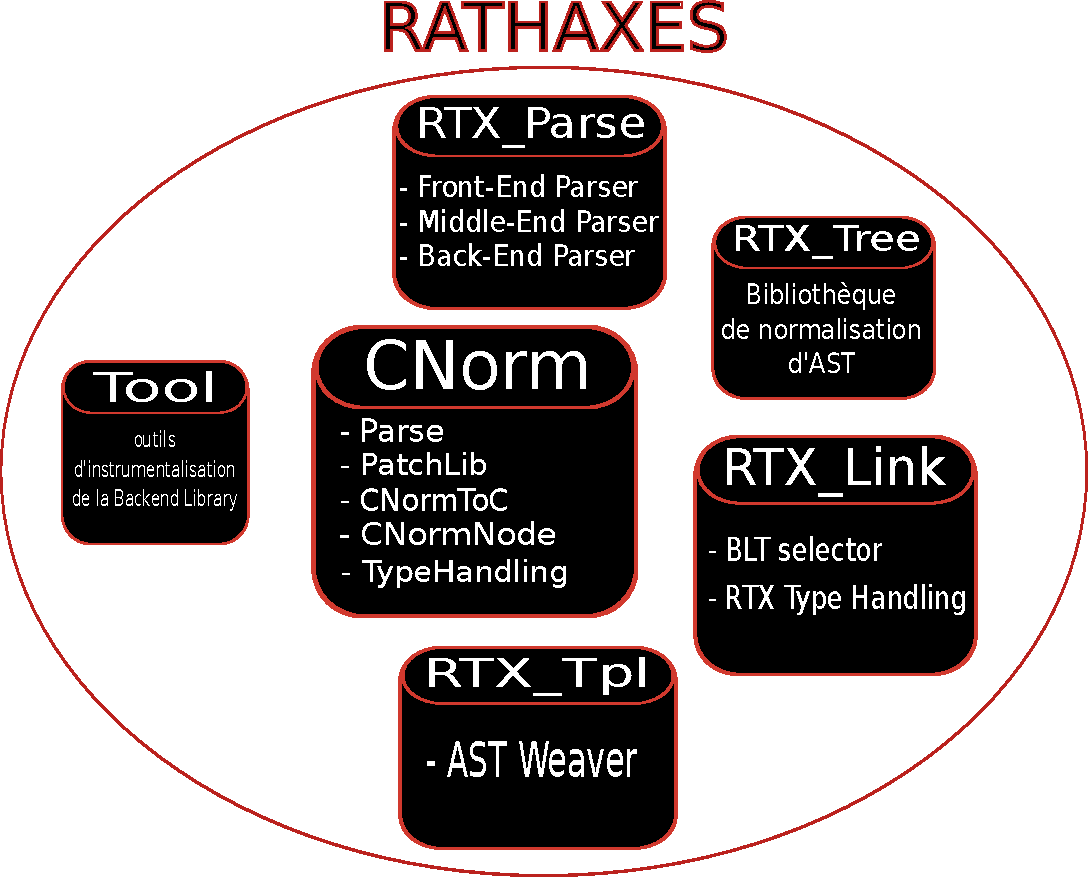
\includegraphics[width=0.95\textwidth]{diagramme_architecture.pdf}

Tout d'abord, la bibliothèque \emph{Cnorm} vue auparavant fait partie du
compilateur. Son rôle est tout d'abord de générer le code C final, mais c'est
aussi ce qui permet l'analyse du code C contenu dans les modèles de code du
backend, grâce aux fonctionnalités de surcharge de syntaxe de CodeWorker.

Le composant suivant, \emph{RTX\_Parse}, est le composant dont le rôle est
(comme son nom l'implique) l'analyse syntaxique de l'ensemble du langage. Il
construit ainsi un arbre de syntaxe abstraite.

\emph{RTX\_Tree} vient avec \emph{RTX\_Parse}, puisque c'est le composant qui
permet de normaliser l'AST généré. Ainsi, chaque type de nœud de l'arbre
respecte un format précis et fixé de représentation de données.

Ensuite, les deux composants \emph{RTX\_Link} et \emph{RTX\_Tpl} sont les
modules qui entrent en jeu lors du processus de transformation d'un AST \rtx en
AST C grâce a l'utilisation des modèles de code. Leur rôle sera détaillé plus
amplement dans la section \ref{sec:compilationSteps}.

Finalement, le module \emph{Tool} est un module plus utilitaire qu'autre chose.
En effet, il contient une série d'outils permettant de générer des fichiers
requis par les systèmes d'exploitation cibles, mais qui ne sont pas exactement
du code C. Par exemple, sur un système du type UNIX, il permettra de générer un
Makefile facilitant la compilation du code du pilote, tandis que sur un système
Windows, il permettra de générer un fichier \texttt{.inf} qui fournit des
information au noyau au sujet du module à charger.


\section{Les étapes de compilation}
\label{sec:compilationSteps}

De l'analyse syntaxique d'un fichier \texttt{.rtx} à la génération du code C
d'un pilote, l'AST va subir un certain nombre de transformations. Cependant,
les templates sont eux aussi compilés dans le but de les sauvegarder dans un
cache au sein du compilateur. Ceci mène à deux modèles de compilation : La
compilation d'un template, et la compilation d'un pilote.

\subsection{Template}

La compilation d'un template peut être divisée en plusieurs étapes, puisque la
compilation d'un template génère une représentation en AST ainsi que du code
CodeWorker. Ce code permettra de faire la résolution de toutes les variables
provenant du frontend lors de l'intégration de la représentation AST du
template au sein de l'AST du pilote.

On peut ainsi identifier les étapes suivantes :
\begin{enumerate}
    \item Analyse syntaxique : construction d'un AST normalisé par le Cnorm et
        RTX\_Tree;
    \item Identification des placeHolders : construction d'une node référençant
        chacun des placeHolder.
    \item Analyse des placeHolders : Construction d'une node pour chacun des
        placeHolders référencés.
    \item Génération de CodeWorker : génération de code CodeWorker dont le rôle
        est de résoudre les placeHolders a l'aide des variables templates
        provenant du frontend, permettant le tissage de l'AST du template dans
        l'AST du pilote final.
\end{enumerate}

Par la suite, le développeur pourra installer le template compilé au sein de la
bibliothèque backend du compilateur. Installer signifie qu'une entrée sera
ajoutée dans un cache au sein du compilateur, permettant de le retrouver lors
de la compilation d'un pilote.


\subsection{Pilote}
\label{sec:driverCompilation}

La compilation d'un pilote est un processus complexe, où chaque partie du DSL
est prise en compte.

Voici une liste des étapes de la compilation d'un pilote :
\begin{enumerate}
    \item Analyse syntaxique : construction d'un AST a partir du code frontend ;
    \item Vérification du typage : vérification des types utilisés dans le
        frontend par rapport aux types fournis par l'interface.
    \item Sélection de template : le composant RTX\_Link sélectionne dans le
        cache les templates correspondant aux variables de configuration
        provenant du frontend ; variables;
    \item Instanciation du template : le composant RTX\_Tpl instancie chaque
        template AST référencé par le frontend, et appelle la fonction
        CodeWorker de résolution des variables templates, avant de lier les
        deux AST ;
    \item Génération : génération du code C à partir de l'AST transformé ;
    \item Génération des outils : Le module \emph{Tool} génère les fichiers
        annexes nécessaires pour la bonne compilation des pilotes générés.
\end{enumerate}


\subsection{Processus de compilation général}

Comme vous avez pu le comprendre, si nous avons parlé de trois parties d'un
seul et même langage, c'est pour la simple et bonne raison que le compilateur
est capable de gérer les trois indifféremment. En effet, on pourrait dans
l'absolu écrire un pilote en partant de rien dans un seul et même fichier.
Cependant, cette possibilité est principalement réservée dans le but de faire
une suite de tests. De plus, les 3 principaux utilisateurs de \rtx se
concentreront normalement chacun sur une des trois parties du langage.

Ceci se ferait donc grâce à l'identification des mots clefs contenus dans le
fichier. Voici un schéma illustrant ce processus général :

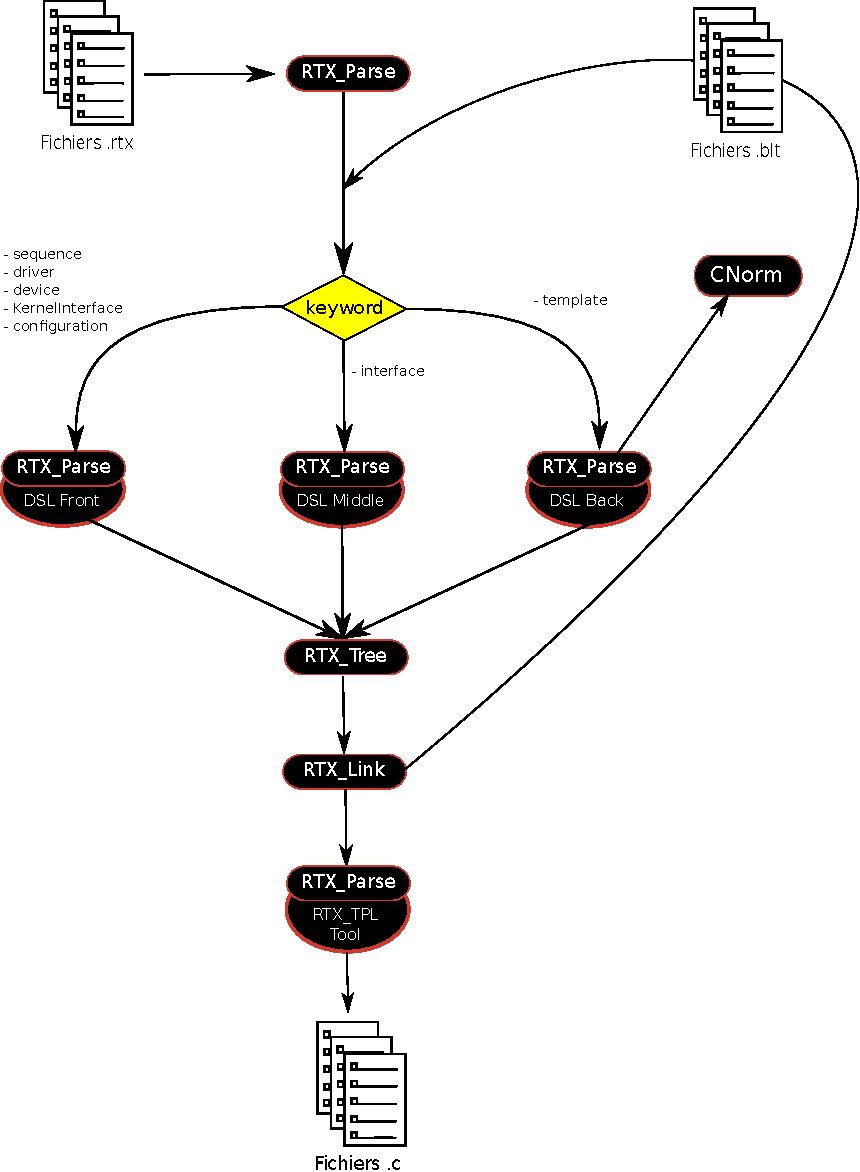
\includegraphics[width=0.95\textwidth]{logigramme.pdf}



\chapter{Détails d'implémentation}



\section{Cache de modèles précompilés}

Un des éléments les plus importants du compilateur est le \emph{cache}. Au
travers de celui-ci, le compilateur peut maintenir une liste complète de
modèles de codes et d'interfaces précompilées, qui permettra de trouver
rapidement les \emph{templates} à utiliser pour la compilation et la génération
d'un pilote.

CodeWorker utilise une variable globale appelée ``this'', où l'on peut stocker
n'importe quelle information. Elle est en réalité utilisée par rathaxes afin de
stocker le \emph{cache} et de le rendre accessible durant toute la phase de
compilation et de génération. Nous y stockons les informations suivantes :
\begin{enumerate}
    \item Les ``codes globaux'' enregistrés
    \item Les \emph{templates} enregistrés
    \item Les \emph{chunks} enregistrés
    \item Un état différentiel du cache
\end{enumerate}

Chacune de ces catégories se traduit par un nœud contenu dans le champ
``session'' de la variable globale ``this'' de CodeWorker. Nous l'appelons la
session de cache.

Tout élément enregistré est un bout de code précompilé et vérifié par le
compilateur avant son enregistrement. Ainsi, chacun d'entre eux est associé à
un fichier de script CodeWorker généré (qui a pour rôle la résolution de tous
les placeholders du code associé) ainsi qu'un fichier \texttt{.tree} contenant
l'AST correspondant. Ces deux éléments peuvent être optionnels pour certains
éléments enregistrés dans le cache.

Maintenant, nous allons décrire chacune de ces catégories de manière plus
détaillée, et expliquer leur rôle et leur utilisation.


\subsection{Codes globaux enregistrés}

Les codes globaux enregistrés sont contenus dans le champ ``.global\_code'' de
la session de cache.

Un ``code global'' est un bout de code spécifique au sein de rathaxes : c'est
une sorte de \emph{chunk} hors d'un \emph{template}, dont la sélection est
automatique dès le moment ou l'interface qui le contient est utilisée pour la
génération d'un pilote. C'est donc du code C instrumenté contenu dans un bloc
\emph{with}.

Seul un élément de cette catégorie peut être chargé pour une interface donnée.
Lors de la génération du pilote, chacun des codes globaux associés à chaque
interface sera automatiquement chargé, résolu et tissé dans l'AST final, dès le
moment où leur interface est utilisée.

Lorsqu'un code global est enregistré dans le cache, il est inséré en tant
qu'élément dans une liste, ou chaque élément contient les champs suivants :
\begin{itemize}
    \item ``.with'': Nœud décrivant les contraintes de configuration
        permettant la sélection du morceau de code (C'est aussi l'élément qui
        indique à quelle interface est associée le code global)
    \item ``.script\_file'': Champ obligatoire.
    \item ``.tree\_file'': Champ obligatoire.
\end{itemize}


\subsection{Template enregistrés}

Les \emph{templates} enregistrés sont contenus dans le champ ``.templates'' de
la session de cache.

Ce champ est en réalité un tableau associatif où la clef est un hash du
prototype du \emph{template}, et la valeur une liste des \emph{templates}
enregistrés associés à ce prototype. Cela permet de pouvoir conserver tous les
\emph{templates}, quelles que soient leurs contraintes de sélection, puis de
faire le tri afin de sélectionner le bon \emph{template} selon la
configuration. Cela dit, deux \emph{templates} enregistrés ne peuvent avoir de
contraintes identiques : Celles-ci doivent différer, et l'on permet ainsi
d'éviter aussi bien des problématiques liées a la sélection du bon
\emph{template}, ainsi que des problématiques liées au double enregistrement
d'un \emph{template}.

Chaque \emph{template} enregistré est un nœud contenant les champs suivants :
\begin{itemize}
    \item ``.with'': Nœud contenant les contraintes de sélection du
        \emph{template}
    \item ``.rtype'': Nœud contenant le prototype du \emph{template} complet
    \item ``.chunks'': Liste d'objets décrivant les \emph{chunks} contenus par
        le \emph{template}.
    \item ``.script\_file'': Champ optionnel. Il n'est présent que dans le cas
        où le \emph{template} est un \emph{template} de type.
    \item ``.tree\_file'': Champ optionnel. Il n'est présent que dans le cas
        où le \emph{template} est un \emph{template} de type.
\end{itemize}

Chaque objet stocké dans le champ ``.chunks'' est un moyen d'indiquer où est
stocké le \emph{chunk} dans le cache. Sa clef est le nom qualifié du
\emph{pointcut} auquel il est associé, et sa valeur est l'index correspondant
au chunk contenu par le \emph{template} dans la liste des \emph{chunks}
associés au \emph{pointcut} donné. Plus d'informations au sujet de la manière
de stocker les \emph{chunks} sont données dans la section suivante.


\subsection{Chunks enregistres}

Les chunks enregistres sont contenus par le champ ``.chunks'' de la session de
cache.

Ce champ est un tableau associatif, qui suit le même modèle que le tableau
associatif qu'est le champ ``.templates''. La clef est le nom du
\emph{pointcut} qualifie (ex: ``interface::nom'' ou ``::nom'' s'il n'est
associe a aucune interface), et la valeur est une liste des \emph{chunks} qui y
sont associes. De la même manière que pour les \emph{templates}, les
\emph{chunks} contenus dans cette liste sont uniques.

Chaque chunk enregistré contient les champs suivants :
\begin{itemize}
    \item ``.with'': Nœud contenant les contraintes de sélection du
        \emph{template} contenant le \emph{chunk}
    \item ``.name'': Nom qualifié du pointcut
    \item ``.tpl\_id'': Hash du \emph{template} contenant le \emph{chunk}
    \item ``.script\_file'': Champ obligatoire.
    \item ``.tree\_file'': Champ obligatoire.
\end{itemize}


\subsection{État Différentiel du cache}

Ce que nous appelons un ``état différentiel du cache'' est en réalité une sorte
de registre de toutes les modifications appliquées au cache durant le processus
de compilation. Ceci permet de pouvoir valider ou non l'enregistrement d'un
élément au sein du cache, et de pouvoir retrouver quels sont les fichiers de
script et d'AST à sauvegarder ou non. C'est ce qui permet l'opération dite
"d'installation" d'un \emph{template} ou d'une interface.

Le différentiel de cache est contenu dans le champ ``.temp'' de la session, et
a une structure similaire à la session de cache elle-même, à cela près que chacun
de ses éléments enregistres est en fait une référence sur l'élément
enregistré dans la session de cache. C'est ce qui permet de les supprimer
facilement, et de les gérer comme n'importe quel élément du cache durant le
processus de génération de pilote.

Lorsque le cache est validé, le compilateur, selon les argument qu'il a reçus,
peut installer les fichiers nouvellement précompilés au sein du cache
persistant. Ce processus d'installation consiste en trois opérations :
\begin{itemize}
    \item Calculer un nom de fichier à partir d'informations associes à
        l'élément à enregistrer
    \item Copier les fichiers précompilés dans la bibliothèque de backend sous
        le nom calculé
    \item Mettre à jour les chemins de fichiers au sein du cache
\end{itemize}

Grâce au différentiel de session, ces opérations sont facilement effectuées, et
le cache peut rester cohérent.


\subsection{API de manipulation du cache}

Dans cette section sont décrites toutes les fonctions ``publiques'' du cache,
de faciliter la maintenance de son code et son utilisation.  Chacune de ces
fonctions se trouve dans le fichier rtxLink.inc.cws des scripts du compilateur.

Tout abord, il est nécessaire de comprendre que le cache a deux possibles cas
d'utilisation : le remplir avec des fichiers que l'on vient de précompiler, ou
en tirer des informations nécessaires à la génération d'un pilote.

\vspace{20pt}

Les fonctions à utiliser pour les deux cas d'utilisation sont les suivantes :

\begin{lstlisting}
function rtxLink_LoadCache();
\end{lstlisting}
La fonction \emph{rtxLink\_LoadCache} est utilisée pour charger le cache en
mémoire depuis un fichier contenant sa description, qui se trouve dans la
bibliothèque de backend. Si cette fonction n'est pas appelée avant un autre
appel au cache, il sera considéré comme vide, et effacera l'ancien cache si il
devait par hasard être sauvegardé.

\begin{lstlisting}
function rtxLink_SaveCache();
\end{lstlisting}
La fonction \emph{rtxLink\_SaveCache} est utilisée pour sauvegarder le cache
dans un fichier situé dans la bibliothèque de backend, afin de le rendre
persistant. Si une quelconque modification a été apportée au cache avant un
appel à cette fonction, elle se chargera automatiquement de sauvegarder les
fichiers temporaires correctement au sein de la bibliothèque du backend et de
mettre à jour le cache persistant.

\begin{lstlisting}
function hashTemplatePrototype(theRType     : node,
                               out_ref_hash : reference);
\end{lstlisting}
La fonction \emph{hashTemplatePrototype} prend en premier argument une node
décrivant le prototype du \emph{template} et en second argument une référence
permettant de renvoyer le hash du prototype. Cette fonction est utilisée de
manière éparse dans le code, afin de maintenir une cohérence dans le hash
utilise pour les \emph{templates}.

\vspace{20pt}

Les fonctions suivantes sont utilisées afin d'insérer des éléments dans le
cache.

\begin{lstlisting}
function rtxLink_RegisterToCache(local_node : node);
\end{lstlisting}
La fonction \emph{rtxLink\_RegisterToCache} traverse un AST rathaxes dans son
ensemble, et enregistre chaque bloc au sein du cache (code global,
\emph{template}, chunks).

\vspace{20pt}

Les fonctions suivantes sont utilisées pour manipuler le cache, afin de
résoudre des placeholders et de générer du code. Nous pouvons alors identifier
quatre cas d'utilisation : Résolution d'un \emph{pointcut} (instanciation de
tous les \emph{chunks} sélectionnés associés), résolution d'un code global,
résolution d'un \emph{chunk} au travers du \emph{template} associé (mécanisme
interne tels que l'appel d'une séquence), et finalement la résolution d'un
mapping de \emph{template} de type.

\begin{lstlisting}
function rtxLink_findGlobalCode(with_values  : node,
                                out_code_ref : reference);
\end{lstlisting}
La fonction \emph{rtxLink\_findGlobalCode} récupère le nœud d'un code global
correspondant à la configuration ``with\_values'' et la retourne grâce à la
référence donnée en second paramètre.

\vspace{20pt}

Fonctions utilisées pour résoudre un \emph{template} (ou un de ses \emph{chunks}) :
\begin{lstlisting}
function rtxLink_findTemplates(theRtype : node,
                               out_tpls : node);
\end{lstlisting}
La fonction \emph{rtxLink\_findTemplates} récupère la liste complète des
\emph{templates} associés à un prototype décrit par le paramètre ``theRtype''
et la copie dans le paramètre ``out\_tpls''.

\begin{lstlisting}
function rtxLink_selectUniqueTemplate(templates : reference,
                                      config : node);
\end{lstlisting}
La fonction \emph{rtxLink\_selectUniqueTemplate} sélectionne un \emph{template}
unique dans la liste de \emph{templates} donnée dans le paramètre ``templates'',
récupérée au travers de la fonction \emph{rtxLink\_findTemplates} en fonction
de la configuration contenue par le paramètre ``config''. Le \emph{template}
sélectionné est alors référencé dans le paramètre ``templates'' pour le retour.
En cas d'échec, la fonction renvoie ``false''.

Dans le cas d'une résolution de mapping de \emph{template} de type, la node ainsi
récupérée peut être directement envoyée à la fonction
\emph{rtxLink\_LoadScript}, qui chargera l'arbre et le script associés.

\begin{lstlisting}
function rtxLink_selectChunkFromTemplate(theTemplate : node,
                                         chunkName : value,
                                         theChunk : reference);
\end{lstlisting}
La fonction \emph{rtxLink\_selectChunkFromTemplate} prend une node de
\emph{template} récupérée grâce à la fonction
\emph{rtxLink\_SelectUniqueTemplate} ainsi qu'un nom qualifié de
\emph{pointcut} par le paramètre ``chunkName''. Elle va alors aller chercher le
\emph{chunk} associé au \emph{template} portant le nom demandé. Si aucun
\emph{chunk} associé ne porte ce nom, elle renvoie ``false''. S'il existe un
\emph{chunk} associé mais qu'il n'est pas trouvé, alors elle renvoie une
exception (c'est un cas qui ne devrait cependant pas être croisé, ou bien votre
cache pourrait être corrompu). Le \emph{chunk} ainsi sélectionné est renvoyé
grâce a la référence ``theChunk''.

Cette fonction est utilisée afin de résoudre un \emph{chunk} précis d'un
\emph{template} donné. Il est ainsi utilisé pour des mécanismes internes et
automatiques du langage (tels que l'appel à un \emph{template} de séquence,
débouchant sur l'instanciation du \emph{chunk} ``::CALL'' associé), ou pour
mapper une fonction membre d'un \emph{template} de type (instanciant ainsi le
\emph{chunk} portant le même nom que la fonction dite ``membre'').

\vspace{20pt}

Fonctions utilisées pour résoudre un \emph{pointcut} :
\begin{lstlisting}
function rtxLink_findChunks(pointcut_name : node,
                            out_chunks : node);
\end{lstlisting}
La fonction \emph{rtxLink\_findChunks} récupère la liste de tous les
\emph{chunks} associés au \emph{pointcut} ``pointcut\_name''. Cette liste est
copiée dans le paramètre ``out\_chunks''.


\begin{lstlisting}
function rtxLink_selectCompatibleChunks(chunks : node,
                                        config : node);
\end{lstlisting}
La fonction \emph{rtxLink\_selectCompatibleChunks} sélectionne les
\emph{chunks} compatibles avec la configuration ``config'' parmi les
\emph{chunks} contenus dans la liste ``chunks'', récupérée au travers de la
fonction \emph{rtxLink\_findChunks}. La liste est alors filtrée pour ne
contenir plus que les \emph{chunks} sélectionnés.

Il est alors possible de transmettre chacun de ces \emph{chunks} à la fonction
\emph{rtxLink\_LoadScript} pour générer du code.


\begin{lstlisting}
function rtxLink_LoadScript(cache_node : node,
                            out_ref_tree : reference);
\end{lstlisting}
La fonction \emph{rtxLink\_LoadScript} charge le script associé à la node, et
l'AST associé dans le paramètre ``out\_ref\_tree''. Elle empêche le
double chargement d'un même script, et ne doit manipuler que des nodes
provenant du cache (donc récupérées au travers des fonctions du cache
précédemment décrites).



%\section{Compilation des Interfaces}

% TODO

\section{Compilation des patrons de code}

\rtx\ reconnait deux types de templates, les templates de \emph{séquences} et
les templates de \emph{type}. Ils partagent les mêmes étapes de compilations:
\begin{enumerate}
    \item Parse : \texttt{rtxParse/rtxBack.inc.cws};
    \item Compile : \texttt{rtxTpl/rtxCompile.inc.cws};
    \item Meta : \texttt{rtxTpl/rtxMeta.inc.cws};
    \item TypeHash : \texttt{rtxTpl/rtxTypeHash.inc.cws};
    \item Introspect : \texttt{rtxTpl/rtxIntrospect.inc.cws};
    \item Gen : \texttt{rtxTpl/rtxGen.inc.cws}.
\end{enumerate}
Cependant, l'étape ---finale--- de génération du code est légèrement différente
pour les templates de type, nous y reviendrons.

Les différentes étapes de compilations aurait pus être faites en une seule passe
sur l'AST, mais pour garder un code facile à maintenir une passe par étape est
réalisée. Le compilateur sépare donc chaque passe dans une fonction template
CodeWorker spécialisée sur le type de nœud traversé. % Cela permet des
% spécialisations utiles pour traverser des types de nœuds différents. Par
% exemple, un nœud qui contient une liste peut parcourir chaque élément qu'elle
% contient; tandis qu'un nœud qui contient deux champs spécifiques peut
% seulement parcourir ces deux champs. Cela permet aussi une gestion spécifique
% des nœuds utiles pour chaque passes.

Voici une description de chacune des étapes appliquées sur l'AST.

\subsection{Parse}

L'étape de parsing construit un AST normalisé avec l'aide du module
\texttt{rtxNode}.

Cette étape est en réalité partagée avec tout ce que \rtx\ accepte en entré. Le
code de parsing se situe dans le répertoire \texttt{rtxParse/}, les fonctions
partagée avec le reste du code sont dans le fichier \texttt{rtxCompile.inc.cwp}
et les règles de parsing spécifiques aux templates sont dans le fichier
\texttt{rtxBack.inc.cwp}.

\subsection{Compile}

Cette étape identifie les parties de codes qui sont instrumentées avec des
\emph{«~placeholders~»}. Chaque placeholder identifié est associé avec les
informations nécessaire pour trouver sa place réelle dans l'AST, puis ajouté
dans une liste nommé \texttt{.compile} dans le nœud racine de C instrumenté.

\subsection{Meta}

Cette étape traverse chaque placeholder identifié à l'étape de compilation.

Chaque placeholder est parsé indépendamment de son contexte et le nœud qui en
résulte est ajouté dans le nœud du même placeholder. Ce nouveau nœud sera
utilisé dans l'étape de génération du code pour enfin résoudre le placeholder.

\subsection{TypeHash}

Cette étape identifie toutes les déclarations de variables \rtx\ et de récupérer
leur nom et leur type.

Ces information permettent de faire référence à des variables \rtx\ depuis des
placeholders et de vérifier leur validité. Elle sont donc stockées dans un nœud
appelé \texttt{.type\_map} pour chaque bloc de code instrumenté
(\emph{«~chunk~»}) puis utilisées lors de résolution des placeholders.

\subsection{Introspect}

Cette étape identifie chaque déclaration de variable de code instrumenté pour
associer les types ---que ce soit des types \rtx\ ou des types
% “base code type” == « types définis dans le code » ?
définis dans le code--- avec leurs variables. Ceci aide l'algorithme de
résolution des placeholders lorsqu'une variable locale est utilisée. % ?

\subsection{Gen}

La dernière étape avant d'enregistrer un template dans le cache du compilateur
est de générer le script CodeWorker qui résout chaque placeholder de chaque bloc
de code instrumenté. Pour chaque bloc de code instrumenté le script contient une
fonction template CodeWorker qui contient les appels pour résoudre chacun de ses
placeholders. Le code généré sera différent selon si le placeholder est la
déclaration d'un type de variable \rtx\ ou d'un \emph{«~pointcut~»}.

Ce script sera utilisé pour obtenir un AST qui pourra être tissé dans le
template appelant.

\subsection{Particularités des templates de types}

% Alors là j'ai eu beaucoup de mal a traduire les ”mapping association” qui se
% traduisent plus ou moins par « association association ».

Le processus de compilation est le même pour les templates de types et les
templates de séquences à la différence près que les templates de type
contiennent un bloc \emph{«~map~»} qui décrit l'association à exposer lors de
l'utilisation de ce type.

De la même manière qu'une fonction est générée pour chaque bloc de code
instrumenté que le template de type contient; une seconde fonction template
CodeWorker est généré pour le block «~map~» du template. Cette fonction gère
chaque association du template et résout chacun d'eux.

La fonction qui génère ce code se nomme «~\texttt{gencodeworker<"\_\_rtx\_tpl\_type\_map\_\_">}~»
et se trouve dans le fichier \texttt{rtxTpl/rtxGen.inc.cws}.

%\section{Compilation d'un pilote}

% TODO

\end{document}
